% Options for packages loaded elsewhere
\PassOptionsToPackage{unicode}{hyperref}
\PassOptionsToPackage{hyphens}{url}
%
\documentclass[
]{article}
\usepackage{lmodern}
\usepackage{amssymb,amsmath}
\usepackage{ifxetex,ifluatex}
\ifnum 0\ifxetex 1\fi\ifluatex 1\fi=0 % if pdftex
  \usepackage[T1]{fontenc}
  \usepackage[utf8]{inputenc}
  \usepackage{textcomp} % provide euro and other symbols
\else % if luatex or xetex
  \usepackage{unicode-math}
  \defaultfontfeatures{Scale=MatchLowercase}
  \defaultfontfeatures[\rmfamily]{Ligatures=TeX,Scale=1}
\fi
% Use upquote if available, for straight quotes in verbatim environments
\IfFileExists{upquote.sty}{\usepackage{upquote}}{}
\IfFileExists{microtype.sty}{% use microtype if available
  \usepackage[]{microtype}
  \UseMicrotypeSet[protrusion]{basicmath} % disable protrusion for tt fonts
}{}
\makeatletter
\@ifundefined{KOMAClassName}{% if non-KOMA class
  \IfFileExists{parskip.sty}{%
    \usepackage{parskip}
  }{% else
    \setlength{\parindent}{0pt}
    \setlength{\parskip}{6pt plus 2pt minus 1pt}}
}{% if KOMA class
  \KOMAoptions{parskip=half}}
\makeatother
\usepackage{xcolor}
\IfFileExists{xurl.sty}{\usepackage{xurl}}{} % add URL line breaks if available
\IfFileExists{bookmark.sty}{\usepackage{bookmark}}{\usepackage{hyperref}}
\hypersetup{
  pdftitle={Agribusiness Management and Cooperative},
  pdfauthor={Deependra Dhakal},
  hidelinks,
  pdfcreator={LaTeX via pandoc}}
\urlstyle{same} % disable monospaced font for URLs
\usepackage[margin=1in]{geometry}
\usepackage{longtable,booktabs}
% Correct order of tables after \paragraph or \subparagraph
\usepackage{etoolbox}
\makeatletter
\patchcmd\longtable{\par}{\if@noskipsec\mbox{}\fi\par}{}{}
\makeatother
% Allow footnotes in longtable head/foot
\IfFileExists{footnotehyper.sty}{\usepackage{footnotehyper}}{\usepackage{footnote}}
\makesavenoteenv{longtable}
\usepackage{graphicx}
\makeatletter
\def\maxwidth{\ifdim\Gin@nat@width>\linewidth\linewidth\else\Gin@nat@width\fi}
\def\maxheight{\ifdim\Gin@nat@height>\textheight\textheight\else\Gin@nat@height\fi}
\makeatother
% Scale images if necessary, so that they will not overflow the page
% margins by default, and it is still possible to overwrite the defaults
% using explicit options in \includegraphics[width, height, ...]{}
\setkeys{Gin}{width=\maxwidth,height=\maxheight,keepaspectratio}
% Set default figure placement to htbp
\makeatletter
\def\fps@figure{htbp}
\makeatother
\setlength{\emergencystretch}{3em} % prevent overfull lines
\providecommand{\tightlist}{%
  \setlength{\itemsep}{0pt}\setlength{\parskip}{0pt}}
\setcounter{secnumdepth}{5}

% use Unicode characters - try changing the option if you run into troubles with special characters (e.g. umlauts)
\usepackage[utf8]{inputenc}

% clean citations
\usepackage{cite}

% hyperref makes references clicky. use \url{www.example.com} or \href{www.example.com}{description} to add a clicky url
\usepackage{nameref,hyperref}

% line numbers
% \usepackage[right]{lineno}

% % improves typesetting in LaTeX
% \usepackage{microtype}
% \DisableLigatures[f]{encoding = *, family = * }

% text layout - change as needed
\raggedright
\setlength{\parindent}{0.5cm}
\textwidth 6.50in % \textwidth 5.25in
\textheight 8.75in % \textheight 8.75in

% use adjustwidth environment to exceed text width (see examples in text)
\usepackage{changepage}

% adjust caption style
\usepackage[aboveskip=1pt,labelfont=bf,labelsep=period,singlelinecheck=off]{caption}

% remove brackets from references
\makeatletter
\renewcommand{\@biblabel}[1]{\quad#1.}
\makeatother


% headrule, footrule and page numbers
\usepackage{fancyhdr}
\pagestyle{fancy}
\fancyfoot[C]{\thepage}
\renewcommand{\headrulewidth}{0.4pt}
\renewcommand{\footrulewidth}{0.6pt}
\newcommand{\TheAuthor}{}
\newcommand{\Author}[1]{\renewcommand{\TheAuthor}{#1}}
\fancyfoot[R]{---~\TheAuthor}
\Author{Deependra Dhakal}

% use \textcolor{color}{text} for colored text (e.g. highlight to-do areas)
\usepackage{color}

% define custom colors (this one is for figure captions)
\definecolor{Gray}{gray}{.25}

% this is required to include graphics
\usepackage{graphicx}

% use if you want to put caption to the side of the figure - see example in text
\usepackage{sidecap}

\newcommand{\blandscape}{\begin{landscape}}
\newcommand{\elandscape}{\end{landscape}}

\usepackage{bm} % for supporting bold math fonts
\usepackage{siunitx}
\usepackage{moreverb}
\usepackage{booktabs}
\usepackage{longtable}
\usepackage{array}
\usepackage{multirow}

% use for have text wrap around figures
\usepackage{wrapfig}
\usepackage[pscoord]{eso-pic}
\usepackage[fulladjust]{marginnote}
\reversemarginpar

\usepackage{float}
\usepackage{colortbl}
\usepackage{pdflscape}
\usepackage{tabu}
\usepackage{threeparttable}
\usepackage{threeparttablex}
\usepackage[normalem]{ulem}
\usepackage{makecell}
\usepackage{xcolor}
\usepackage{tikz} % required for image opacity change
\usepackage[absolute,overlay]{textpos} % for text formatting
\usepackage{chemfig}

\newcommand\BibTeX{{\rmfamily B\kern-.05em \textsc{i\kern-.025em b}\kern-.08em
T\kern-.1667em\lower.7ex\hbox{E}\kern-.125emX}}
\sisetup{per-mode=symbol}

% this is to sort and place the reference in nice order
\DeclareRobustCommand{\firstsecond}[2]{#2}

% \bibliographystyle{plainnat}
\usepackage[numbers]{natbib}

% Added by CII
% \usepackage[format=hang,labelfont=bf,margin=0.5cm,justification=centering]{caption} # don't use bf
\usepackage[format=hang,margin=0.5cm,justification=centering]{caption}
\captionsetup{font=small,width=0.9\linewidth,labelfont=small,textfont={small}}
% End of CII addition

\usepackage{subcaption}
% \newcommand{\subfloat}[2][need a sub-caption]{\subcaptionbox{#1}{#2}}

% \captionsetup[sub]{font=footnotesize}
\captionsetup[subfigure]{font=small,labelfont=small,textfont=small}

% to modify title
\usepackage{titling}
\posttitle{\par\end{center}} % tighten title
\setlength{\droptitle}{-30pt} % remove extra space above title

% coffee spill
\input fun-coffee
\usepackage{everypage}
\usepackage{pgf}

\pgfmathsetseed{\pdfuniformdeviate 10000000}

\pgfmathdeclarerandomlist{scales}{{1}{1.2}{1.6}{1.8}}
\pgfmathdeclarerandomlist{stains}{{\coffeeA}{\coffeeB}{\coffeeC}{\coffeeD}}

\AddEverypageHook{%
  \pgfmathrandominteger{\angle}{15}{350}%
  \pgfmathparse{rand/2.4}\xdef\xoffset{\pgfmathresult}%
  \pgfmathparse{rand/2.4}\xdef\yoffset{\pgfmathresult}%
  \pgfmathparse{(0.1 + rnd/3)}\xdef\trans{\pgfmathresult}%
  \pgfmathrandomitem{\scale}{scales}%
  \pgfmathrandomitem{\stain}{stains}%
  \edef\coffeescale{\trans}\stain%
}

\title{Agribusiness Management and Cooperative}
\usepackage{etoolbox}
\makeatletter
\providecommand{\subtitle}[1]{% add subtitle to \maketitle
  \apptocmd{\@title}{\par {\large #1 \par}}{}{}
}
\makeatother
\subtitle{Practical}
\author{Deependra Dhakal}
\date{11/30/2020}

\begin{document}
\maketitle

{
\setcounter{tocdepth}{1}
\tableofcontents
}
\clearpage

\hypertarget{determination-of-optimum-input-use-and-maximization-of-profit-using-one-input}{%
\section{Determination of optimum input use and maximization of profit using one input}\label{determination-of-optimum-input-use-and-maximization-of-profit-using-one-input}}

\hypertarget{objectives}{%
\subsection*{Objectives}\label{objectives}}
\addcontentsline{toc}{subsection}{Objectives}

\begin{itemize}
\tightlist
\item
  To determine optimum input use and maximize profit using one input
\end{itemize}

\textbf{Numerical}

\begin{enumerate}
\def\labelenumi{\arabic{enumi}.}
\tightlist
\item
  For the following hypothetical data showing input-output relationship between number of tractor plus driver units recruits and hectares of land ploughed, determine.
\end{enumerate}

\begin{table}[H]

\caption{\label{tab:tractor-driver-unit-cmr-tab}Input-output relationship between number of tractor plus driver unit recruits and hectares of land ploughed.}
\centering
\fontsize{8}{10}\selectfont
\begin{tabular}[t]{cc}
\toprule
tractor driver unit & field ploughed\\
\midrule
1 & 2\\
2 & 4\\
5 & 10\\
6 & 12\\
\bottomrule
\end{tabular}
\end{table}

\begin{enumerate}
\def\labelenumi{\alph{enumi}.}
\tightlist
\item
  Which is input ?
\item
  Which is output ?
\item
  Marginal rate of returns at each level of input
\item
  What is the relationship between input-output ?
\end{enumerate}

\begin{enumerate}
\def\labelenumi{\arabic{enumi}.}
\setcounter{enumi}{1}
\tightlist
\item
  For the following hypothetical data showing input-output relationship between wheat seed used per hectare and wheat production, determine.
\end{enumerate}

\begin{table}[H]

\caption{\label{tab:nitrogen-wheat-imr-tab}Marginal rate of return for hypothetical wheat production scenario.}
\centering
\fontsize{8}{10}\selectfont
\begin{tabular}[t]{rlrl}
\toprule
wheat seed & marginal wheat seed & wheat production & marginal wheat production\\
\midrule
10 &  & 1000 & \\
15 &  & 1025 & \\
20 &  & 1075 & \\
25 &  & 1150 & \\
30 &  & 1250 & \\
\addlinespace
35 &  & 1375 & \\
\bottomrule
\end{tabular}
\end{table}

\begin{enumerate}
\def\labelenumi{\alph{enumi}.}
\tightlist
\item
  Which is input ?
\item
  Which is output ?
\item
  Marginal rate of returns at each level of input
\item
  Trend of marginal rate of return
\end{enumerate}

\begin{enumerate}
\def\labelenumi{\arabic{enumi}.}
\setcounter{enumi}{2}
\tightlist
\item
  For the following hypothetical data showing input-output relationship between fertilizer use in wheat per hectare and wheat production, determine.
\end{enumerate}

\begin{table}[H]

\caption{\label{tab:nitrogen-wheat-dmr-tab}Marginal rate of return for hypothetical wheat production scenario.}
\centering
\fontsize{8}{10}\selectfont
\begin{tabular}[t]{rlrl}
\toprule
wheat fertilizer & marginal wheat fertilizer & wheat production & marginal wheat production\\
\midrule
100 &  & 2000 & \\
150 &  & 2600 & \\
200 &  & 3100 & \\
250 &  & 3500 & \\
300 &  & 3800 & \\
\addlinespace
350 &  & 4000 & \\
\bottomrule
\end{tabular}
\end{table}

\begin{enumerate}
\def\labelenumi{\alph{enumi}.}
\tightlist
\item
  Which is input ?
\item
  Which is output ?
\item
  Marginal rate of returns at each level of input
\item
  Trend of marginal rate of return
\end{enumerate}

\clearpage

\hypertarget{determination-of-least-cost-combination-of-inputs-using-graphical-and-arithmetic-method}{%
\section{Determination of least cost combination of inputs using graphical and arithmetic method}\label{determination-of-least-cost-combination-of-inputs-using-graphical-and-arithmetic-method}}

\hypertarget{objectives-1}{%
\subsection*{Objectives}\label{objectives-1}}
\addcontentsline{toc}{subsection}{Objectives}

\begin{itemize}
\tightlist
\item
  To graphically represent cost combinations for two inputs
\item
  To arithmetically determine the least cost combination of inputs
\end{itemize}

\textbf{Numerical}

\begin{enumerate}
\def\labelenumi{\arabic{enumi}.}
\tightlist
\item
  For the following hypothetical data showing relationship between two fertilizers (Nitrogen and Phosphorus) used in Wheat crop to produce common yield of 2 tons per hectare, determine:
\end{enumerate}

\begin{table}[H]
\centering\begingroup\fontsize{8}{10}\selectfont

\begin{tabular}{lrrrrr}
\toprule
Yield & Nitrogen ($X_2$) & Phosphorus ($X_1$) & $\Delta X_2$ & $\Delta X_1$ & MRS ($\frac{\Delta X_2}{\Delta X_1}$)\\
\midrule
\cellcolor{gray!6}{2 tons} & \cellcolor{gray!6}{46} & \cellcolor{gray!6}{0} & \cellcolor{gray!6}{} & \cellcolor{gray!6}{} & \cellcolor{gray!6}{}\\
2 tons & 32 & 2 & -14 & 2 & 7.0\\
\cellcolor{gray!6}{2 tons} & \cellcolor{gray!6}{20} & \cellcolor{gray!6}{4} & \cellcolor{gray!6}{-12} & \cellcolor{gray!6}{2} & \cellcolor{gray!6}{6.0}\\
2 tons & 10 & 6 & -10 & 2 & 5.0\\
\cellcolor{gray!6}{2 tons} & \cellcolor{gray!6}{1} & \cellcolor{gray!6}{8} & \cellcolor{gray!6}{-9} & \cellcolor{gray!6}{2} & \cellcolor{gray!6}{4.5}\\
\addlinespace
2 tons & 0 & 10 & -1 & 2 & 0.5\\
\bottomrule
\end{tabular}
\endgroup{}
\end{table}

\begin{enumerate}
\def\labelenumi{\alph{enumi}.}
\tightlist
\item
  Marginal rate of input substitution of nitrogen for phosphorus
\item
  Graph showing cost combination of inputs and the least cost combination point.
\item
  Calculate the least cost combination of input use using arithmetic method if the price of Phosphorus is Rs 40/kg and price of Nitrogen is Rs 20/kg.
\end{enumerate}

\clearpage

\hypertarget{determination-of-optimum-enterprise-combination-for-revenue-maximization}{%
\section{Determination of optimum enterprise combination for revenue maximization}\label{determination-of-optimum-enterprise-combination-for-revenue-maximization}}

\hypertarget{objectives-2}{%
\subsection*{Objectives}\label{objectives-2}}
\addcontentsline{toc}{subsection}{Objectives}

\begin{itemize}
\tightlist
\item
  To maximize revenue through optimum enterprise combination
\end{itemize}

\textbf{Numerical}

For the given hypothetical data on alternative combinations of Rice and Wheat enterprise using same amount of resources, determine:

\begin{table}[H]

\caption{\label{tab:pp-schedule}Production possibility schedule}
\centering
\fontsize{8}{10}\selectfont
\begin{tabular}[t]{>{\centering\arraybackslash}p{10em}>{\centering\arraybackslash}p{10em}>{\centering\arraybackslash}p{10em}}
\toprule
Alternative outputs & Rice (tons) & Wheat (tons)\\
\midrule
\cellcolor[HTML]{FECE91}{\textcolor{white}{\textbf{A}}} & \bgroup\fontsize{8}{10}\selectfont \textcolor[HTML]{440154}{\textbf{0}}\egroup{} & \bgroup\fontsize{16}{18}\selectfont \textcolor[HTML]{7AD151}{\textbf{20}}\egroup{}\\
\cellcolor[HTML]{F2645C}{\textcolor{white}{\textbf{B}}} & \bgroup\fontsize{10}{12}\selectfont \textcolor[HTML]{453882}{\textbf{2}}\egroup{} & \bgroup\fontsize{15}{17}\selectfont \textcolor[HTML]{4CC26C}{\textbf{18}}\egroup{}\\
\cellcolor[HTML]{A1307E}{\textcolor{white}{\textbf{C}}} & \bgroup\fontsize{12}{14}\selectfont \textcolor[HTML]{2A788E}{\textbf{5}}\egroup{} & \bgroup\fontsize{14}{16}\selectfont \textcolor[HTML]{1F9F88}{\textbf{14}}\egroup{}\\
\cellcolor[HTML]{461078}{\textcolor{white}{\textbf{D}}} & \bgroup\fontsize{15}{17}\selectfont \textcolor[HTML]{4CC26C}{\textbf{9}}\egroup{} & \bgroup\fontsize{10}{12}\selectfont \textcolor[HTML]{3C508B}{\textbf{6}}\egroup{}\\
\cellcolor[HTML]{000004}{\textcolor{white}{\textbf{E}}} & \bgroup\fontsize{16}{18}\selectfont \textcolor[HTML]{7AD151}{\textbf{10}}\egroup{} & \bgroup\fontsize{8}{10}\selectfont \textcolor[HTML]{440154}{\textbf{0}}\egroup{}\\
\bottomrule
\end{tabular}
\end{table}

\begin{enumerate}
\def\labelenumi{\arabic{enumi}.}
\tightlist
\item
  Graphically show production possibility frontier.
\item
  Which type of product combination is indicated ?
\item
  Using arithmetic method determine optimum production with combination of enterprises. Assume that price of Rice is Rs 20/kg and price of Wheat is Rs 30/kg.
\end{enumerate}

\clearpage

\hypertarget{farm-record-keeping-and-preparation-of-farm-inventory}{%
\section{Farm record keeping and preparation of farm inventory}\label{farm-record-keeping-and-preparation-of-farm-inventory}}

\hypertarget{objectives-3}{%
\subsection*{Objectives}\label{objectives-3}}
\addcontentsline{toc}{subsection}{Objectives}

\begin{itemize}
\tightlist
\item
  To understand usefulness and purpose of keeping farm record
\item
  To be able to maintain farm inventory of an operating farm
\end{itemize}

\hypertarget{introduction}{%
\subsection*{Introduction}\label{introduction}}
\addcontentsline{toc}{subsection}{Introduction}

Farm accounting and record keeping is a science of recording farm business transaction. It helps to understand nature and the extent of the financial effects. Records are important in analyzing farm business to understand the fairness of business and its weakness and improvements needed.

\textbf{Advantages of farm records and accounts}

\begin{itemize}
\tightlist
\item
  Means to higher income
\item
  Basis for diagnosis and planning
\item
  Way to improve managerial skills of farmer
\item
  Basis for credit acquisition and management
\item
  Guide to better home management
\item
  Basis for conducting research in agricultural and production economics
\item
  Basis for government policies
\end{itemize}

General forms of farm record are:

\begin{enumerate}
\def\labelenumi{\arabic{enumi}.}
\tightlist
\item
  Farm inventory
\item
  Farm cash accounts or farm financial accounts
\item
  Classified farm cash account and annual farm business analysis
\item
  Supplementary financial records (Capital assets sale register; cash sale register; credit sale/purchase register; wage register; funds borrowed, repayments register, farm expenses register, non-farm income record)
\end{enumerate}

\hypertarget{farm-inventory}{%
\subsubsection*{Farm inventory}\label{farm-inventory}}
\addcontentsline{toc}{subsubsection}{Farm inventory}

It is a list of the whole physical property of a business along with their values at a specified date. It is the complete list of farmers' assets. It is the first step in farm accounting. For an illustration, see Table \ref{tab:farm-inventory-ex}.

\begingroup\fontsize{8}{10}\selectfont

\begin{longtable}[t]{>{\raggedright\arraybackslash}p{8em}>{\raggedright\arraybackslash}p{6em}>{\raggedright\arraybackslash}p{6em}>{\raggedright\arraybackslash}p{5em}>{\raggedright\arraybackslash}p{5em}>{\raggedright\arraybackslash}p{5em}>{\raggedright\arraybackslash}p{5em}}
\caption{\label{tab:farm-inventory-ex}Farm inventory of Betaaleshwor agro farm on Baisakh 2076 and Chaitra 2076}\\
\toprule
\multicolumn{3}{c}{ } & \multicolumn{2}{c}{Beginning of 2076} & \multicolumn{2}{c}{End of 2076} \\
\cmidrule(l{3pt}r{3pt}){4-5} \cmidrule(l{3pt}r{3pt}){6-7}
 &  & Item & Quantity & Value & Quantity & Value\\
\midrule
 & Crop produce &  & 0.0 & 0 & 0 & 0\\
\cmidrule{2-7}\nopagebreak
 &  & Seeds & 0.0 & 0 & 0 & 0\\
\cmidrule{3-7}\nopagebreak
 &  & Urea (fertilizer) & 5.0 & 200 & 2 & 80\\
\cmidrule{3-7}\nopagebreak
 &  & DAP (fertilizer) & 2.0 & 120 & 1 & 60\\
\cmidrule{3-7}\nopagebreak
 &  & MoP (fertilizer) & 0.0 & 0 & 1 & 55\\
\cmidrule{3-7}\nopagebreak
 &  & BHC 10\% (Pesticide) & 0.5 & 25 & 0 & 0\\
\cmidrule{3-7}\nopagebreak
 &  & Blitox (Pesticide) & 2.0 & 240 & 0 & 0\\
\cmidrule{3-7}\nopagebreak
 & \multirow{-7}{*}{\raggedright\arraybackslash Supplies} & Malthion (Pesticide) & 2.5 & 300 & 1 & 120\\
\cmidrule{2-7}\nopagebreak
 & Maize seed (Crop growing) &  & 3.0 & 600 & 3 & 600\\
\cmidrule{2-7}\nopagebreak
 & Sugarcane setts (Crop growing) &  & 100.0 & 1000 & 100 & 1000\\
\cmidrule{2-7}\nopagebreak
 & Marketable livestock &  & 0.0 & 0 & 0 & 0\\
\cmidrule{2-7}\nopagebreak
\multirow{-12}{*}{\raggedright\arraybackslash Non depreciable assets} & Others &  & 0.0 & 0 & 0 & 0\\
\cmidrule{1-7}\pagebreak[0]
 &  & Tractor & 1.0 & 250000 & 1 & 200000\\
\cmidrule{3-7}\nopagebreak
 &  & Tiller, disc harrow & 1.0 & 50000 & 1 & 45000\\
\cmidrule{3-7}\nopagebreak
 &  & Tubewell & 1.0 & 20000 & 1 & 19000\\
\cmidrule{3-7}\nopagebreak
 &  & Trolley & 1.0 & 25000 & 1 & 22500\\
\cmidrule{3-7}\nopagebreak
 &  & Wheat thresher & 1.0 & 22600 & 1 & 20000\\
\cmidrule{3-7}\nopagebreak
 &  & Seed cum fertilizer drill & 1.0 & 22500 & 1 & 20400\\
\cmidrule{3-7}\nopagebreak
 & \multirow{-7}{*}{\raggedright\arraybackslash Farm machinery} & Other implements and hand tools (bulk unit) & 1.0 & 15000 & 1 & 12000\\
\cmidrule{2-7}\nopagebreak
 & Farm buildings &  & 1.0 & 300000 & 1 & 280000\\
\cmidrule{2-7}\nopagebreak
 & Livestock (buffaloes, cattle) (number) &  & 12.0 & 400000 & 12 & 300000\\
\cmidrule{2-7}\nopagebreak
\multirow{-10}{*}{\raggedright\arraybackslash Depreciable assets} & Land (ha) &  & 2.0 & 2400000 & 2 & 2400000\\
\cmidrule{1-7}\pagebreak[0]
 & Cash in hand &  &  & 15000 &  & 12500\\
\cmidrule{2-7}\nopagebreak
 & Small savings or bank deposits &  &  & 120000 &  & 90000\\
\cmidrule{2-7}\nopagebreak
 & Shares in cooperatives &  &  & 5000 &  & 5000\\
\cmidrule{2-7}\nopagebreak
\multirow{-4}{*}{\raggedright\arraybackslash Cash assets} & Other properties &  &  & 0 &  & 0\\
\bottomrule
\end{longtable}
\endgroup{}

\begin{table}[!h]

\caption{\label{tab:farm-inventory-summary}Change in inventory}
\centering
\begin{tabular}[t]{lr}
\toprule
record date & value\\
\midrule
Beginning of year 2076 & 3647585\\
End of year 2076 & 3428315\\
Change & 219270\\
\bottomrule
\end{tabular}
\end{table}

\clearpage

\hypertarget{calculation-of-depreciation-of-farm-assets}{%
\section{Calculation of depreciation of farm assets}\label{calculation-of-depreciation-of-farm-assets}}

\hypertarget{objectives-4}{%
\subsection*{Objectives}\label{objectives-4}}
\addcontentsline{toc}{subsection}{Objectives}

\begin{itemize}
\tightlist
\item
  To know different methods of calculation of depreciation
\end{itemize}

Decline in the value of an asset or capital equipment due to wear and tear of the asset, time, damages. Whenever any machines or equipment performs useful work, its wear and tear is bound to occur. Its efficiency reduces and becomes uneconomical to be used further and needs replacement by another new one.

\textbf{Concepts of depreciation}

\begin{itemize}
\tightlist
\item
  Original cost of asset: Bought price or purchasing cost of asset.
\item
  Salvage value: The expected recovery of sales value of the asset at the end of useful life. (purchase value of asset/ expected life of that asset)
\item
  Useful life: The expected time period for which the asset is to provide economic service i.e.~the period for which the asset could be used for production.
\item
  Depreciable cost: The original cost minus salvage value.
\item
  Written down value: The value of asset at any point of time is the original cost less accumulated depreciation to date.
\end{itemize}

\textbf{Methods of computing depreciation}

\begin{enumerate}
\def\labelenumi{\arabic{enumi}.}
\tightlist
\item
  Annual re-evaluation
\item
  Straight line method
\item
  Diminishing balance method
\item
  Sum of the year-digit method or reducing fraction method
\item
  Compound interest method
\end{enumerate}

\hypertarget{numerical}{%
\subsection*{Numerical}\label{numerical}}
\addcontentsline{toc}{subsection}{Numerical}

\begin{enumerate}
\def\labelenumi{\arabic{enumi}.}
\tightlist
\item
  (Using diminishing balance method) Calculate anuual depreciation for a tractor costing Rs. 240000 at the rate of 20\%.
\end{enumerate}

\emph{Solution}

We go on taking 20\% of the remaining balance until salvage value is reached, as in this case this is about Rs. 40330.

\begin{table}[!h]

\caption{\label{tab:unnamed-chunk-2}Computation of annual depreciation by Diminishing balance method}
\centering
\fontsize{8}{10}\selectfont
\begin{tabular}[t]{rrrr}
\toprule
Year & Value at the beginning of year & Annual depreciation & Remaining balance\\
\midrule
\cellcolor{gray!6}{1} & \cellcolor{gray!6}{240000} & \cellcolor{gray!6}{48000} & \cellcolor{gray!6}{192000}\\
2 & 192000 & 38400 & 153600\\
\cellcolor{gray!6}{3} & \cellcolor{gray!6}{153600} & \cellcolor{gray!6}{30720} & \cellcolor{gray!6}{122880}\\
4 & 122880 & 24576 & 98304\\
\cellcolor{gray!6}{5} & \cellcolor{gray!6}{98304} & \cellcolor{gray!6}{19661} & \cellcolor{gray!6}{78643}\\
\addlinespace
6 & 78643 & 15729 & 62915\\
\cellcolor{gray!6}{7} & \cellcolor{gray!6}{62915} & \cellcolor{gray!6}{12583} & \cellcolor{gray!6}{50332}\\
8 & 50332 & 10066 & 40265\\
\cellcolor{gray!6}{9} & \cellcolor{gray!6}{40265} & \cellcolor{gray!6}{} & \cellcolor{gray!6}{}\\
\bottomrule
\end{tabular}
\end{table}

\clearpage

\hypertarget{preparation-of-balance-sheet-of-a-farm}{%
\section{Preparation of Balance sheet of a farm}\label{preparation-of-balance-sheet-of-a-farm}}

\hypertarget{objectives-5}{%
\subsection*{Objectives}\label{objectives-5}}
\addcontentsline{toc}{subsection}{Objectives}

\begin{itemize}
\tightlist
\item
  To prepare balance sheet of a farm
\end{itemize}

\hypertarget{introduction-1}{%
\subsection*{Introduction}\label{introduction-1}}
\addcontentsline{toc}{subsection}{Introduction}

The balance sheet, also called net worth or financial statement, is a summary of assets and liabilities of a business together with the statement of the owners' equity or net worth. This is a listing of all assets and liabilities of a farm at certain point of time. This reports the financial strength and progress of the business. The term balance here implies that the value of the assets must be equal to the value fo liabilities plus owner's equity or net worth.

\begin{minipage}[c]{\textwidth}
\scalebox{0.8}{\noindent\begin{minipage}{0.3\textwidth}
\raggedleft
\begin{itemize}
\item Net worth or equity or net assets or capital of a company/farm is calculated by calculating the difference between the Total Assets and the Total Liabilities.
\item An example Net worth statement of MudnBrick Commercial Vegetable and Livestock Farm is presented in Table \ref{tab:net-worth-state}.
\end{itemize}
\end{minipage}}
\scalebox{1.0}{\noindent\begin{minipage}{0.7\textwidth}

\begin{table}[H]

\caption{\label{tab:net-worth-state}Net worth statement}
\centering
\fontsize{8}{10}\selectfont
\begin{tabular}[t]{llll}
\toprule
\multicolumn{4}{c}{\textbf{MudnBrick Commercial Vegetable and Livestock Farm}} \\
\cmidrule(l{3pt}r{3pt}){1-4}
\multicolumn{4}{c}{\em{Financial condition as of 2011-11-11}} \\
\cmidrule(l{3pt}r{3pt}){1-4}
\multicolumn{4}{c}{\textbf{Net Worth Statement}} \\
\cmidrule(l{3pt}r{3pt}){1-4}
 &  &  \vphantom{1}& \\
\midrule
\cellcolor{gray!6}{Assets} & \cellcolor{gray!6}{Market value} & \cellcolor{gray!6}{Liabilities} & \cellcolor{gray!6}{Amount}\\
\multicolumn{1}{c}{\textbf{Current}} & \multicolumn{1}{c}{\textbf{}} & \multicolumn{1}{c}{\textbf{Short-term}} & \multicolumn{1}{c}{\textbf{}}\\
\cellcolor{gray!6}{Cash in hand} & \cellcolor{gray!6}{450} & \cellcolor{gray!6}{Accounts payable} & \cellcolor{gray!6}{14000}\\
Checking/savings & 500 & Unpaid taxes and interest & 35000\\
\cellcolor{gray!6}{Inventory} & \cellcolor{gray!6}{9000} & \cellcolor{gray!6}{Veterinary fees} & \cellcolor{gray!6}{0}\\
\addlinespace
Accounts receivables & 8000 & Other short term loan & 9000\\
\cellcolor{gray!6}{Cash at bank} & \cellcolor{gray!6}{5000} & \cellcolor{gray!6}{} & \cellcolor{gray!6}{}\\
\multicolumn{1}{c}{\textbf{Current total}} & \multicolumn{1}{c}{\textbf{22950}} & \multicolumn{1}{c}{\textbf{Short-term total}} & \multicolumn{1}{c}{\textbf{58000}}\\
\cellcolor{gray!6}{Non-current/Fixed} & \cellcolor{gray!6}{} & \cellcolor{gray!6}{Long term} & \cellcolor{gray!6}{}\\
Farm real estate & 150000 & Farm real estate & 90000\\
\addlinespace
\cellcolor{gray!6}{Tractor} & \cellcolor{gray!6}{1500} & \cellcolor{gray!6}{Automobile loan} & \cellcolor{gray!6}{20000}\\
Farm equipments & 13000 & Building depreciation & 400\\
\cellcolor{gray!6}{Personal property} & \cellcolor{gray!6}{5000} & \cellcolor{gray!6}{Farm animal purchase loan} & \cellcolor{gray!6}{12000}\\
Farm animals and livestocks & 14000 &  & \\
\cellcolor{gray!6}{Non-current/Fixed total} & \cellcolor{gray!6}{183500} & \cellcolor{gray!6}{Long term total} & \cellcolor{gray!6}{122400}\\
\addlinespace
Investment/Long term &  &  \vphantom{1}& \\
\cellcolor{gray!6}{Stocks} & \cellcolor{gray!6}{1000} & \cellcolor{gray!6}{} & \cellcolor{gray!6}{}\\
Bonds & 100 &  & \\
\cellcolor{gray!6}{Goodwill} & \cellcolor{gray!6}{5000} & \cellcolor{gray!6}{} & \cellcolor{gray!6}{}\\
Cash value of livestock insurance & 4000 &  & \\
\addlinespace
\cellcolor{gray!6}{Investment/Long term total} & \cellcolor{gray!6}{10100} & \cellcolor{gray!6}{} & \cellcolor{gray!6}{}\\
 &  &  & \\
\cellcolor{gray!6}{Total assets} & \cellcolor{gray!6}{216550} & \cellcolor{gray!6}{Total liabilities} & \cellcolor{gray!6}{180400}\\
\multicolumn{1}{c}{\textbf{Net worth}} & \multicolumn{1}{c}{\textbf{36150}} & \multicolumn{1}{c}{\textbf{}} & \multicolumn{1}{c}{\textbf{}}\\
\bottomrule
\end{tabular}
\end{table}

\end{minipage}}
\end{minipage}

\clearpage

\hypertarget{preparation-of-income-statement-of-a-farm}{%
\section{Preparation of Income statement of a farm}\label{preparation-of-income-statement-of-a-farm}}

\hypertarget{objectives-6}{%
\subsection*{Objectives}\label{objectives-6}}
\addcontentsline{toc}{subsection}{Objectives}

\begin{itemize}
\tightlist
\item
  To be able to prepare an Income statement of a farm
\end{itemize}

\hypertarget{introduction-2}{%
\subsection*{Introduction}\label{introduction-2}}
\addcontentsline{toc}{subsection}{Introduction}

Balance sheet shows only the amount of wealth held by a business at one moment in time. Profit generated during a period is a main concern of many users of financial statements. P\&L statement provides a picture of profitability of the farm -- How much wealth (that is, profit) was generated, or lost, by the business over that period?

Profit (loss) is defined as the increase (decrease) in wealth arising from trading activities. This is more accurately done using an accrual statement, which further accounts for inventory, accounts payable, and receivables, as well as depreciation expense. The difference between the total revenue and total expenses will represent either profit (if revenue exceeds expenses) or loss (if expenses exceed revenue). The period over which profit or loss is normally measured is usually known as the ``accounting period'', or ``financial period''.

\begin{table}[H]

\caption{\label{tab:cost-return-an}Income statement}
\centering
\fontsize{8}{10}\selectfont
\begin{tabular}[t]{lll}
\toprule
\multicolumn{3}{c}{\textbf{Income statement}} \\
\cmidrule(l{3pt}r{3pt}){1-3}
\em{\textbf{}} & \em{\textbf{Particulars}} & \em{\textbf{Amount (Rs./ropani/annum)}}\\
\midrule
\cellcolor{gray!6}{1} & \cellcolor{gray!6}{Sales revenue of vegetables and dairy product} & \cellcolor{gray!6}{\textcolor[HTML]{BBDF27}{\textbf{55000}}}\\
2 & Less cost of sales (Marketing, transport, etc.) & \textcolor[HTML]{46065A}{\textbf{1200}}\\
\cellcolor{gray!6}{} & \cellcolor{gray!6}{Gross profit} & \cellcolor{gray!6}{\textcolor[HTML]{ADDC30}{\textbf{53800}}}\\
1 & Less salaries and wages payment of farm keepers & \textcolor[HTML]{2D708E}{\textbf{22514}}\\
\cellcolor{gray!6}{2} & \cellcolor{gray!6}{Less heat and light cost} & \cellcolor{gray!6}{\textcolor[HTML]{46065A}{\textbf{1200}}}\\
\addlinespace
3 & Less insurance & \textcolor[HTML]{481E70}{\textbf{5331.6}}\\
\cellcolor{gray!6}{4} & \cellcolor{gray!6}{Less motor vehicle running expenses} & \cellcolor{gray!6}{\textcolor[HTML]{460B5E}{\textbf{2200}}}\\
5 & Less depreciation - fixtures and fittings & \textcolor[HTML]{450457}{\textbf{800}}\\
\cellcolor{gray!6}{6} & \cellcolor{gray!6}{Less depreciation - Vehicles} & \cellcolor{gray!6}{\textcolor[HTML]{440154}{\textbf{400}}}\\
\multicolumn{1}{c}{\textbf{}} & \multicolumn{1}{c}{\textbf{Operating profit}} & \multicolumn{1}{c}{\textbf{\textcolor[HTML]{2F6B8E}{\textbf{21354.4}}}}\\
\addlinespace
\cellcolor{gray!6}{1} & \cellcolor{gray!6}{Interest received from investments} & \cellcolor{gray!6}{\textcolor[HTML]{460A5D}{\textbf{2000}}}\\
2 & Less interest on borrowings & \textcolor[HTML]{450457}{\textbf{900}}\\
\cellcolor{gray!6}{} & \cellcolor{gray!6}{Profit for the period} & \cellcolor{gray!6}{\textcolor[HTML]{2D708E}{\textbf{22454.4}}}\\
\bottomrule
\end{tabular}
\end{table}

\clearpage

\hypertarget{calculation-of-farm-efficiency-measures}{%
\section{Calculation of farm efficiency measures}\label{calculation-of-farm-efficiency-measures}}

\hypertarget{objectives-7}{%
\subsection*{Objectives}\label{objectives-7}}
\addcontentsline{toc}{subsection}{Objectives}

\begin{itemize}
\tightlist
\item
  Analyzing both physical and financial efficiency measures
\end{itemize}

\hypertarget{introduction-3}{%
\subsection*{Introduction}\label{introduction-3}}
\addcontentsline{toc}{subsection}{Introduction}

\emph{Efficiency ratios}

\begin{enumerate}
\def\labelenumi{\arabic{enumi}.}
\tightlist
\item
  Land use efficiency
\end{enumerate}

\[\text{Production efficiency} = \frac{\text{Yield of the crop in a farm}}{\text{Average yield of the locality}}\]

\[\text{Cropping intensity} = \frac{\text{Area cropped}}{\text{Total cultivated area}}\]

\[\text{System index} = \frac{\text{Potential net income per hectare on farm}}{\text{Average standard net income per hectare in the area}} \times 100\]

\begin{enumerate}
\def\labelenumi{\arabic{enumi}.}
\setcounter{enumi}{1}
\tightlist
\item
  Labor efficiency measures
\end{enumerate}

\begin{itemize}
\tightlist
\item
  Crop acres per man or per man-year
\item
  Livestock maintained per man or per man-year
\item
  Gross profit per man or per man-year
\end{itemize}

\begin{enumerate}
\def\labelenumi{\arabic{enumi}.}
\setcounter{enumi}{2}
\tightlist
\item
  Machinery efficiency
\end{enumerate}

\begin{itemize}
\tightlist
\item
  Machinery and equipment cost per cropped acre
\item
  Investment in machinery and equipment per crop acre
\end{itemize}

\emph{Cost ratios}

\begin{enumerate}
\def\labelenumi{\arabic{enumi}.}
\tightlist
\item
  Operating ratio: Represents the proportion absorbed by operating expenses out of the gross income.
\end{enumerate}

\[\text{Operating cost ratio} = \frac{\text{Total operating cost or farm expenses}}{\text{Total profit or gross farm income}}\]

\begin{enumerate}
\def\labelenumi{\arabic{enumi}.}
\setcounter{enumi}{1}
\tightlist
\item
  Fixed ratio
\end{enumerate}

\[\text{Fixed ratio (aka. Overhead charges ratio)} = \frac{\text{Total fixed cost per year}}{\text{Gross income}}\]

\begin{enumerate}
\def\labelenumi{\arabic{enumi}.}
\setcounter{enumi}{2}
\tightlist
\item
  Gross ratio
\end{enumerate}

\[\text{Gross ratio} = \frac{\text{Total farm expenses}}{\text{Total cash expenses}}\]

\begin{enumerate}
\def\labelenumi{\arabic{enumi}.}
\setcounter{enumi}{3}
\tightlist
\item
  Expense structure ratio
\end{enumerate}

\[\text{Expense structure ratio} = \frac{\text{Fixed cash expenses}}{\text{Total cash expenses}}\]

\emph{Profitability ratios}

\begin{enumerate}
\def\labelenumi{\arabic{enumi}.}
\tightlist
\item
  Capital turnover ratio
\item
  Rate of return on debit and equity capital
\item
  Rate of return on equity capital
\end{enumerate}

\clearpage

\hypertarget{representation-of-production-chain-market-chain-and-supply-chain-in-a-value-chain-map-of-an-agricultural-commodity}{%
\section{Representation of production chain, market chain and supply chain in a value chain map of an agricultural commodity}\label{representation-of-production-chain-market-chain-and-supply-chain-in-a-value-chain-map-of-an-agricultural-commodity}}

\hypertarget{objectives-8}{%
\subsection*{Objectives}\label{objectives-8}}
\addcontentsline{toc}{subsection}{Objectives}

\begin{itemize}
\tightlist
\item
  To represent graphically the production chain, market chain and supply chain in a value chain map of an agricultural commodity
\end{itemize}

\hypertarget{introduction-4}{%
\subsection*{Introduction}\label{introduction-4}}
\addcontentsline{toc}{subsection}{Introduction}

Porter (1985) defined value chain is a chain of activities. Products pass through all activities of the chain in order and at each activity the product gains some value. The value chain categorizes the generic value adding activities of an organization.

A value chain map graphically illustrates all of the components, and relationships between them. Value chain maps demonstrate how a product in an industry moves from raw material through production, processing, and other steps, until it eventually ends with the consumer.

\hypertarget{value-chain-map-of-ginger-produced-in-sindhuli-district}{%
\subsection*{Value chain map of ginger produced in Sindhuli district}\label{value-chain-map-of-ginger-produced-in-sindhuli-district}}
\addcontentsline{toc}{subsection}{Value chain map of ginger produced in Sindhuli district}

\begin{center}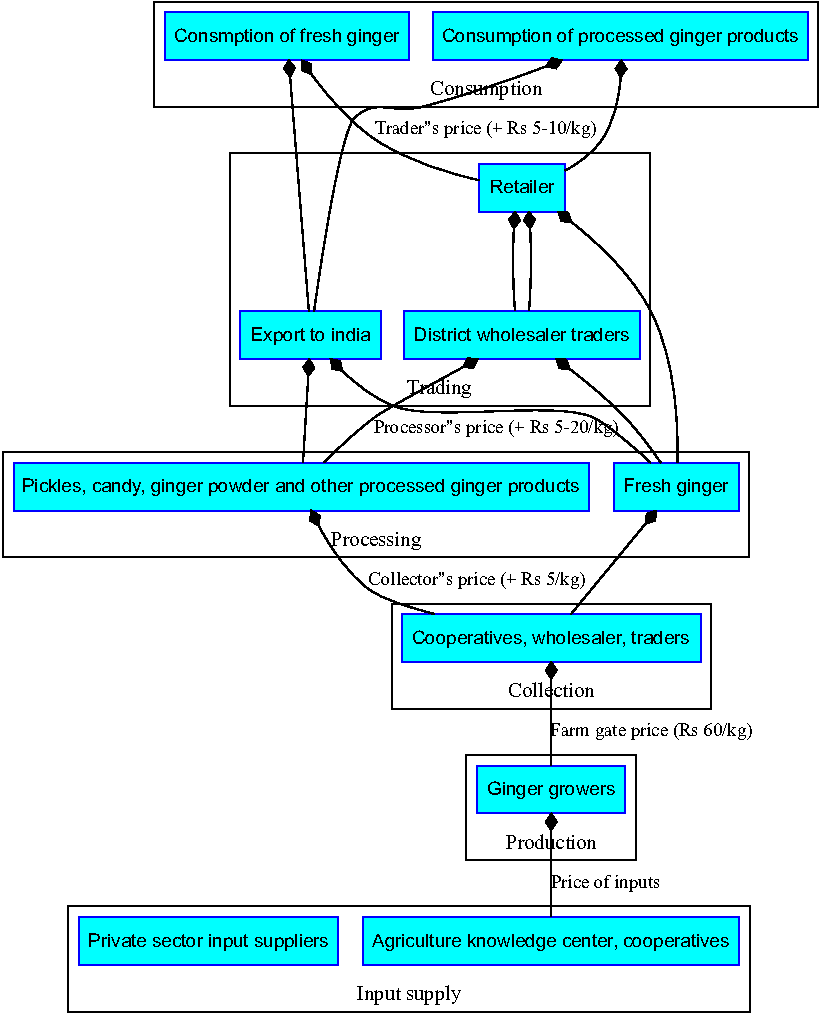
\includegraphics[width=0.6\linewidth]{practicals_files/figure-latex/diagram-value-chain-ginger-1} \end{center}

\clearpage

\hypertarget{determination-of-project-worth-using-investment-appraisal-criteria}{%
\section{Determination of project worth using investment appraisal criteria}\label{determination-of-project-worth-using-investment-appraisal-criteria}}

\hypertarget{objectives-9}{%
\subsection*{Objectives}\label{objectives-9}}
\addcontentsline{toc}{subsection}{Objectives}

\begin{itemize}
\tightlist
\item
  To determine projects' worth using investment appraisal criteria
\end{itemize}

\end{document}
